\documentclass[10pt,twocolumn]{article} 
\usepackage{style}
\usepackage{times}
\usepackage{graphicx}
\usepackage{amssymb}
\usepackage{url,hyperref}
\usepackage{orcidlink}
\usepackage{amsmath}

% Remove borders around links
\usepackage{xcolor}
\hypersetup{
	colorlinks,
	linkcolor={red!50!black},
	citecolor={blue!50!black},
	urlcolor={blue!80!black}
}

\begin{document}
	
	\title{\emph{Binary Search}: An Implementation Guide}
	
	\author{Kunal K. Singh \orcidlink{0009-0008-6906-2062}  \\
		\\
		Technical Report \\
		Bhopal, MP, India \\
		\today
		\\
		\\
		kunalsin9h@gmail.com  \\
	}
	
	\maketitle
	\thispagestyle{empty}
	
	\begin{abstract}
		Binary Search is on the most popular \emph{searching} algorithms. It is used in variety of applications, but implementing it requires careful consideration of various components like \emph{lower} and \emph{upper} bounds, \emph{mid} value, conditions and answers. I present a general method of \textbf{implementing} binary search. This process always give the correct result and it is very easy to work with. We have focused more on implementation then explaining different binary search concepts. 
	\end{abstract}
	
	
	\section{Introduction}
	%	We can classify Binary Search into two sub-classes, Finding \textbf{First True} or \textbf{Last True}. All binary search problems will more or less belong to one the two mentioned categories. 
		
		Binary search is a highly efficient searching algorithm that operates on \textit{\textbf{sorted collections}} of data, employing a \textit{\textbf{divide-and-conquer}} strategy by systematically dividing the search space in half until the target element is found. The algorithm maintains two essential components: the \texttt{lower} and \texttt{upper} bounds, which define the current search space. 
		
		\begin{center}
			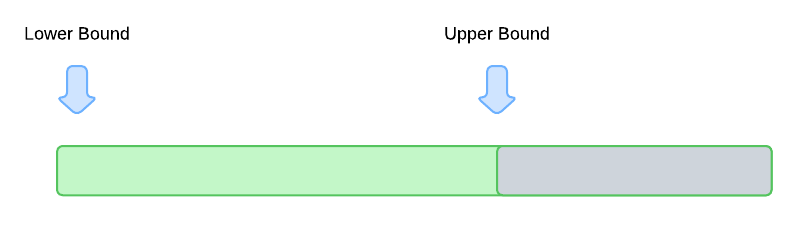
\includegraphics[width=0.5\textwidth]{bounds.png}
		\end{center}
		
		These boundaries are dynamically adjusted as the search progresses, with the lower bound typically starting at the first index and the upper bound at the last index of the array.
		
		
		The algorithm's effectiveness relies on the \textbf{predicate function}, which evaluates positions within the search space and returns a boolean value to determine the target's location relative to the current position. This function must maintain monotonically to establish a clear \texttt{true/false} boundary across the search space.
		
	 	Binary search achieves logarithmic time complexity \texttt{O(log n)} by eliminating half of the remaining search space in each iteration, making it particularly valuable in applications such as database index lookups, sorted array searching, and optimization problems where the search space can be represented as a sorted sequence.
	 	
	 	An common implementation of binary search goes like:
	 	
	 	\vspace{10pt}
	 	
	 	\noindent
	 	\textbf{Algorithm:} Binary Search\\
	 	1. \textbf{Input:} \(key, array\) \\
	 	2. \textbf{Output:} \(index\) \\
	 	3. \(lower \gets 0\) \\
	 	4. \(upper \gets len(array) - 1\) \\
	 	5. \textbf{while} \(lower \leq upper\) \textbf{ do} \\
	 	6. \quad\(mid \gets (lower + upper) / 2\) \\
	 	7. \quad \textbf{if} \(array[mid] = key \) \textbf{ then} \\
	 	8. \quad \quad Return \(mid\) \\
	 	9. \quad \textbf{if} \(array[mid] > key \) \textbf{ then} \\
	 	10. \quad \quad \(upper \gets mid - 1\) \\
	 	11. \quad \textbf{else} \\
	 	12. \quad \quad \(lower \gets mid + 1\) \\
	 	13. Return \(-1\)
	 	
	 	\vspace{10pt}
		
		While implementing Binary Search, we may face few problems, they are:
	
	\begin{description}
		\item[$\bullet$]  What is the value of \texttt{lower bound}?
		\item[$\bullet$]  What is the value of \texttt{upper bound}?
		\item[$\bullet$]  How do I calculate my \texttt{mid} value?
		\item[$\bullet$]  What condition should I write in my \texttt{while loop}?
		\item[$\bullet$]  When my predicate is true, should I assign my \texttt{mid} to \texttt{lower} or \texttt{upper} bound?
		\item[$\bullet$]  Whats my final answer, value of \texttt{lower} or \texttt{upper} bound?
	\end{description}
	
	These question are very common while implementing binary search, many times we do mistake and we have to do some debugging to land on correct implementation.
	
	Lets see how we use the presented method for implementing binary search in a generalized manner to achieve consistency and correctness.
	
	\section{First True Binary Search}
	
	The first true binary search is a method for identifying the first element in a sorted list that evaluates to true when tested with a given predicate function.	
	
	\vspace{10pt}
	
	Formally, 
	
	\vspace*{5pt}
	$FirstTrue(A, P) = min\{x \in A: P(x) = true\}$
	\vspace*{5pt}
	
	Where:
	
			\quad$A$ is sorted array / list
		
			\quad$P$ is the predicate function
		
			\quad$min(...)$ finds the smallest element satisfying the condition
			
			
		
	\vspace{10pt}
	
	Graphically,
	
	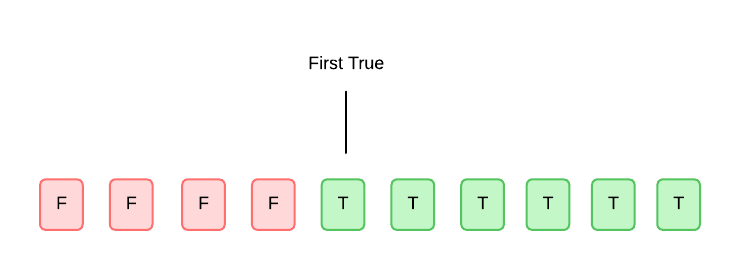
\includegraphics[width=0.5\textwidth]{firsttrue.png}
	
	I present a generalized algorithm implementation method \emph{first true binary search}, with changes from the classic implementation as:
	
	\vspace{5pt}
	
	1. Set \texttt{lower} bound value to be \emph{minimum possible answer}, for an sorted array we can say $0$ ($0th$ index).
	
	2. Set \texttt{upper} bound value to be \emph{maximum possible answer} + $1$, for an sorted array we can say:
	
	\begin{center}
		
	\quad \(maxAnswer \gets len(array) - 1\) \\
	\quad \(upper \gets maxAnswer + 1\) \\ 
	\quad \(upper \gets len(array)\) \\		
	
	
	\end{center}
	
	3. Always use $lower < upper$ as \textbf{condition} in \texttt{while} loop.
	
	4. Find \(mid\) value as normal:
	
	\begin{center}
		$mid \gets (lower + upper) / 2$
	\end{center}
	

	5. If \textbf{predicate} function gives $true$ then set \(high\)  to \(mid\) else set \(lower\) to \(mid + 1\).
	
	6. Answer is always the value of \(lower\) bound.
	
	\vspace*{5pt}
	
	The complete algorithm goes like:
	
	\vspace*{10pt}
	
	\noindent
	\textbf{Algorithm:} Binary Search (First True)\\
	1. \textbf{Input:} \(key, array\) \\
	2. \textbf{Output:} \(index\) \\
	3. \(lowestPossibleAnswer \gets 0\) \\
	4. \(highestPossibleAnswer \gets len(array) - 1\) \\
	5. \(lower \gets lowestPossibleAnswer\) \\
	6. \(upper \gets highestPossibleAnswer + 1\) \\
	7. \textbf{while} \(low < high\) \textbf{ do} \\
	8. \quad\(mid \gets (low + high) / 2\) \\
	9. \quad \textbf{if} \(P(array, key, mid) = true \) \textbf{ then} \\
	10. \quad \quad \(upper \gets mid\) \\
	11. \quad \textbf{else} \\
	12. \quad \quad \(lower \gets mid + 1\) \\
	13. Return \(lower\)
	
	\vspace{10pt}
	
	Where:
	
	\quad $P$ is a predicate function, which returns $true / flase$, in case of sorted array, we can define function $P$ as:

\[
P(array, key, mid) = 
\begin{cases} 
	\text{True} & \text{if } array[mid] \ge key \\ 
	\text{False} & \text{otherwise} 
\end{cases}
\]
	\vspace{5pt}
	
	Hence, following these rules we will always implement a correct binary search algorithm in case of first true.  
		 
	\section{Last True Binary Search}
	
		The last true binary search is a method for identifying the last element in a sorted list that evaluates to true when tested with a given predicate function.	
	
	\vspace{10pt}
	
	Formally, 
	
	\vspace*{5pt}
	$LastTrue(A, P) = max\{x \in A: P(x) = true\}$
	\vspace*{5pt}
	
	Where:
	
	\quad$A$ is sorted array / list
	
	\quad$P$ is the predicate function
	
	\quad$max(...)$ finds the largest element satisfying the condition
	
	
	
	\vspace{10pt}
	
	Graphically,
	
	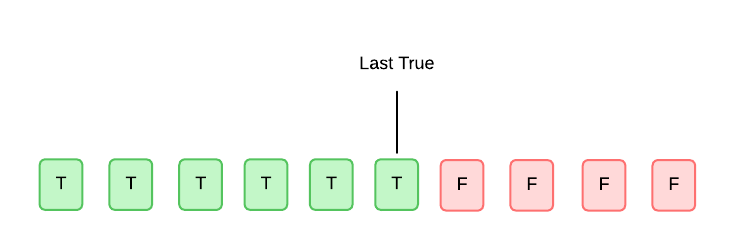
\includegraphics[width=0.5\textwidth]{lasttrue.png}
	
	The generalized algorithm implementation method \emph{last true binary search}, with changes from the classic implementation as:
	
	\vspace{5pt}
	
	1. Set \texttt{lower} bound value to be \emph{minimum possible answer} - \(1\), for an sorted array we can say $-1$.
	
		\begin{center}
		
		\quad \(minAnswer \gets 0\) \\
		\quad \(lower \gets minAnswer - 1\) \\ 
		\quad \(lower \gets -1\) \\		
		
		
	\end{center}
	
	2. Set \texttt{upper} bound value to be \emph{maximum possible answer}, for an sorted array we can say $len(array) - 1$:
	
	3. Always use $lower < upper$ as \textbf{condition} in \texttt{while} loop.
	
	4. Find \(mid\) value with adding $1$:
	
	\begin{center}
		$mid \gets (lower + upper + 1) / 2$
	\end{center}
	
	
	5. If \textbf{predicate} function gives $true$ then set \(low\)  to \(mid\) else set \(upper\) to \(mid - 1\).
	
	6. Answer is always the value of \(lower\) bound.
	
	\vspace*{5pt}
	
	The complete algorithm goes like:
	
	\vspace*{10pt}
	
	\noindent
	\textbf{Algorithm:} Binary Search (Last True)\\
	1. \textbf{Input:} \(key, array\) \\
	2. \textbf{Output:} \(index\) \\
	3. \(lowestPossibleAnswer \gets 0\) \\
	4. \(highestPossibleAnswer \gets len(array) - 1\) \\
	5. \(lower \gets lowestPossibleAnswer - 1\) \\
	6. \(upper \gets highestPossibleAnswer\) \\
	7. \textbf{while} \(low < high\) \textbf{ do} \\
	8. \quad\(mid \gets (low + high + 1) / 2\) \\
	9. \quad \textbf{if} \(P(array, key, mid) = true \) \textbf{ then} \\
	10. \quad \quad \(lower \gets mid\) \\
	11. \quad \textbf{else} \\
	12. \quad \quad \(upper \gets mid - 1\) \\
	13. Return \(lower\)
	
	\vspace{10pt}
	
	Where:
	
	\quad $P$ is a predicate function, which returns $true / flase$, in case of sorted array, we can define function $P$ as:
	
	\[
	P(array, key, mid) = 
	\begin{cases} 
		\text{True} & \text{if } array[mid] < key \\ 
		\text{False} & \text{otherwise} 
	\end{cases}
	\]
	\vspace{5pt}
	
	Again, same as \emph{first true}, following these rules we will always implement a correct binary search algorithm in case of last true.  
	
	\section{The Conclusions}
	
	In conclusion, we can say following these methods for implementing will grantees us the correctness of algorithms. We no longer need to worry about the different components involved in binary search algorithm, and can solely focus on refining the \textbf{predicate} function. You can create a template for reusing it multiple times.
	
	\section{Future Work}
	
	There are two things I would like to explore in future, the generalization of binary search involving \emph{floating point} precision. And writing \textbf{proof} of correctness for these methods. 
	
	\section{Acknowledgment}
	
	This work is inspired from the code submitted by Benq (a top rated competitive programmer) on Codeforces. \href{https://codeforces.com/submissions/Benq}{Here is the link to submitted solutions}.
	
\end{document}